%%%%%%%%%%%%%%%%%%%%%%%%%%%%%%%%%%%%%%%%%%%%%%%%%%%%%%%%%%%%%%%%%%%%%%%%%%%%%%%%
%2345678901234567890123456789012345678901234567890123456789012345678901234567890
%        1         2         3         4         5         6         7         8

%\documentclass[letterpaper, 10 pt, conference]{ieeeconf}  % Comment this line out
                                                          % if you need a4paper
\documentclass[a4paper, 10pt, conference]{ieeeconf}      % Use this line for a4
                                                          % paper

\IEEEoverridecommandlockouts                              % This command is only
                                                          % needed if you want to
                                                          % use the \thanks command
\overrideIEEEmargins
% See the \addtolength command later in the file to balance the column lengths
% on the last page of the document



% The following packages can be found on http:\\www.ctan.org
%\usepackage{graphics} % for pdf, bitmapped graphics files
%\usepackage{epsfig} % for postscript graphics files
%\usepackage{mathptmx} % assumes new font selection scheme installed
%\usepackage{times} % assumes new font selection scheme installed
%\usepackage{amsmath} % assumes amsmath package installed
%\usepackage{amssymb}  % assumes amsmath package installed
\usepackage{graphicx}
\usepackage{subfig}
\usepackage{apacite}
\usepackage{siunitx}
\usepackage{authblk}

\makeatletter
\newcommand*\titleheader[1]{\gdef\@titleheader{#1}}
\AtBeginDocument{%
  \let\st@red@title\@title
  \def\@title{%
    \bgroup\normalfont\large\centering\@titleheader\par\egroup
    \vskip1.5em\st@red@title}
}
\makeatother


\titleheader{GEO441 Remote Sensing Seminar, spring semester 2022}

\title{\huge \bf
Detecting the irrigation cycle of rice fields in the Camargue using time series of Landsat 8 and Sentinel-1
}

%\author{ \parbox{3 in}{\centering Huibert Kwakernaak*
%         \thanks{*Use the $\backslash$thanks command to put information here}\\
%         Faculty of Electrical Engineering, Mathematics and Computer Science\\
%         University of Twente\\
%         7500 AE Enschede, The Netherlands\\
%         {\tt\small h.kwakernaak@autsubmit.com}}
%         \hspace*{ 0.5 in}
%         \parbox{3 in}{ \centering Pradeep Misra**
%         \thanks{**The footnote marks may be inserted manually}\\
%        Department of Electrical Engineering \\
%         Wright State University\\
%         Dayton, OH 45435, USA\\
%         {\tt\small pmisra@cs.wright.edu}}
%}


\author[ ]{Maurus Feyen}
\author[ ]{Yelu He}
\author[ ]{Carola Moos}
\affil[ ]{\textit{Remote Sensing Laboratories, Department of Geography, University of Zurich}}

\begin{document}
\pagenumbering{arabic}


\maketitle
\thispagestyle{plain}
\pagestyle{plain}


%%%%%%%%%%%%%%%%%%%%%%%%%%%%%%%%%%%%%%%%%%%%%%%%%%%%%%%%%%%%%%%%%%%%%%%%%%%%%%%%
\begin{abstract}

The rice fields in the Camargue are the most important rice supplier of France and offer a temporary habitat to migrating bird species during the winter. To detect the crop cycle of rice with its three characteristic periods (irrigation, vegetation growth and harvest) is therefore of interest for the agriculture sector and the biodiversity in the Camargue. Landsat 8 images from 2015 – 2019 were used to generate the indices Normalized Difference Vegetation Index (NDVI), Normalized Difference Water Index (NDWI) and Land Surface Water Index (LSWI). Combined with the SAR backscatter of Sentinel-1 data, the indices were used to detect areas with a clear irrigation pattern to distinguish rice fields from other land cover types. The results of two example plots showed a clear seasonal pattern in one (plot west) while the other (plot east) was not clearly classified as a rice field by our method. Both, however, showed clear patterns of irrigation during some years with the combination of indices and SAR backscatter. The results show that the NDVI, NDWI and SAR backscatter detected the irrigation cycle and vegetation growth very well, while the harvest was not visible in the SAR backscatter. Further research would be needed to map rice fields in the Camargue reliably over the entire growing season.


\end{abstract}


%%%%%%%%%%%%%%%%%%%%%%%%%%%%%%%%%%%%%%%%%%%%%%%%%%%%%%%%%%%%%%%%%%%%%%%%%%%%%%%%
\section{INTRODUCTION}

Rice fields are one of the most distinguishing features of the landscape in the Camargue. They are not only an important supplier of rice in France, but also offer a temporary habitat to various bird species during winter \cite{Pernollet2015ARegimes}. Rice cultivation is crucial to the region to make it cultivable for different crops as it desalinizes the land, durum wheat being the most common to follow rice \cite{Mouret2004AnFrance,Bazzi2019MappingFrance}. The cultivation of rice is possible in the Camargue because of an irrigation network, that uses the water from the Rhône to flood the fields in between 24 April and 16 May \cite{Ndikumana2018EstimationFrance} using pumps and small canals \cite{Grillas1990DistributionFactors, Pernollet2015ARegimes}. Lying in the south-east of France, the region is a dynamic area strongly shaped by the Rhône delta and numerous lagoons. The Camargue has therefore been strongly influenced by the dynamic of desalting and salinizing effects due to alternate flooding \cite{PerennouLaPerspectives, Grillas1990DistributionFactors}. In recent time, this effect has been diminished because of the construction of hydroelectric dams, yet the desalinizing effects of rice is still needed for the agriculture. Mapping the distribution of rice fields and its vegetation cycle is therefore of interest for the agriculture sector and the biodiversity in the Camargue.

There are three characteristic periods of rice fields: flooding, vegetation growth and harvest. During the flooding there is an open water surface, followed by the vegetation growth period where the open water surface mixes with rice crops and finally, the end of harvest that is characterized by bare soil. Remote sensing has been used in various studies to map rice fields based on these characteristics \cite{Xiao2005MappingImages, Li2018MappingOLI, Perennou2018MappingMap, Bazzi2019MappingFrance}. They used different vegetation indices (Normalized Difference Vegetation Index (NDVI) and Enhanced Vegetation Index (EVI)) and the Land Surface Water Index (LSWI) that reflect the seasonal changes in land cover of rice fields (from fallow to flooding to the growing period of rice) \cite{Li2018MappingOLI, Xiao2005MappingImages}. The method was applied in southern China with MODIS images \cite{Xiao2005MappingImages} and the Camargue with Landsat 8 images \cite{Li2018MappingOLI}. The problem with MODIS images is the low spatial resolution of 500 m that can result in an overestimation of rice fields. In this paper we used Landsat 8 images that have a spatial resolution of 30 m. As optical data is dependent on a clear sky and sunlight, the use of Synthetic Aperture Radar (SAR) data has a high potential for a continuous monitoring of rice fields \cite{Bazzi2019MappingFrance}. 

This paper combines time series of Landsat 8 data from 2015–2019 and Sentinel-1 backscatter signatures from 2015–2018 to detect the three phases of rice fields. First, the temporal changes of the multispectral indices over the whole region of interest (ROI) (Figure 1) were analyzed over all land cover types to detect a seasonal pattern of irrigation. Then, we combined the results with the backscattering from Sentinel-1 images. To get a more precise result of the irrigation phase, we then focused on two areas that were regularly classified as rice fields during the previous steps or by the OSO Land Cover Map. Finally, we compared the two areas based on their indices and SAR backscatter to see if there is a similar seasonality in irrigation.
inally, we compared the two rice fields to see if there is a similar seasonality in irrigation.

\section{STUDY SITE}

The study site (Figure \ref{fig:studysite}) lies in the north of the Camargue region in France (centered on 43°36'N and 4°35'E). Most of the area is covered either by heathland, water or agriculture, with tubers and rice as the dominant cultures (Figure \ref{fig:landcover}). According to these land cover classes, we decided for an agricultural area where we could expect many rice fields. It was important to have a part of the river Rhône in the scene, which could be used as a simple validation area when trying to extract water surfaces.

To get a purer result and avoid the mixed signals from other crops, we later focused on two plots within our study site to see if our approach confirms them as rice fields and to get a clear seasonality of irrigation. One area (Plot West) lies in the north-west of the study site and was classified as a rice field regularly by our method although being classified as heathland in the OSO Land Cover Map. The other area (Plot East) lies in the east and is classified as a rice field by the OSO Land Cover Map (Figure \ref{fig:twoplots}). 

\begin{figure}[h]
\centering
\includegraphics[width=8cm]{Figures/Study_site.png}
\caption{Location of our study site. Background: Open Street Map.}
\label{fig:studysite}
\end{figure}

\begin{figure}[h]
\centering
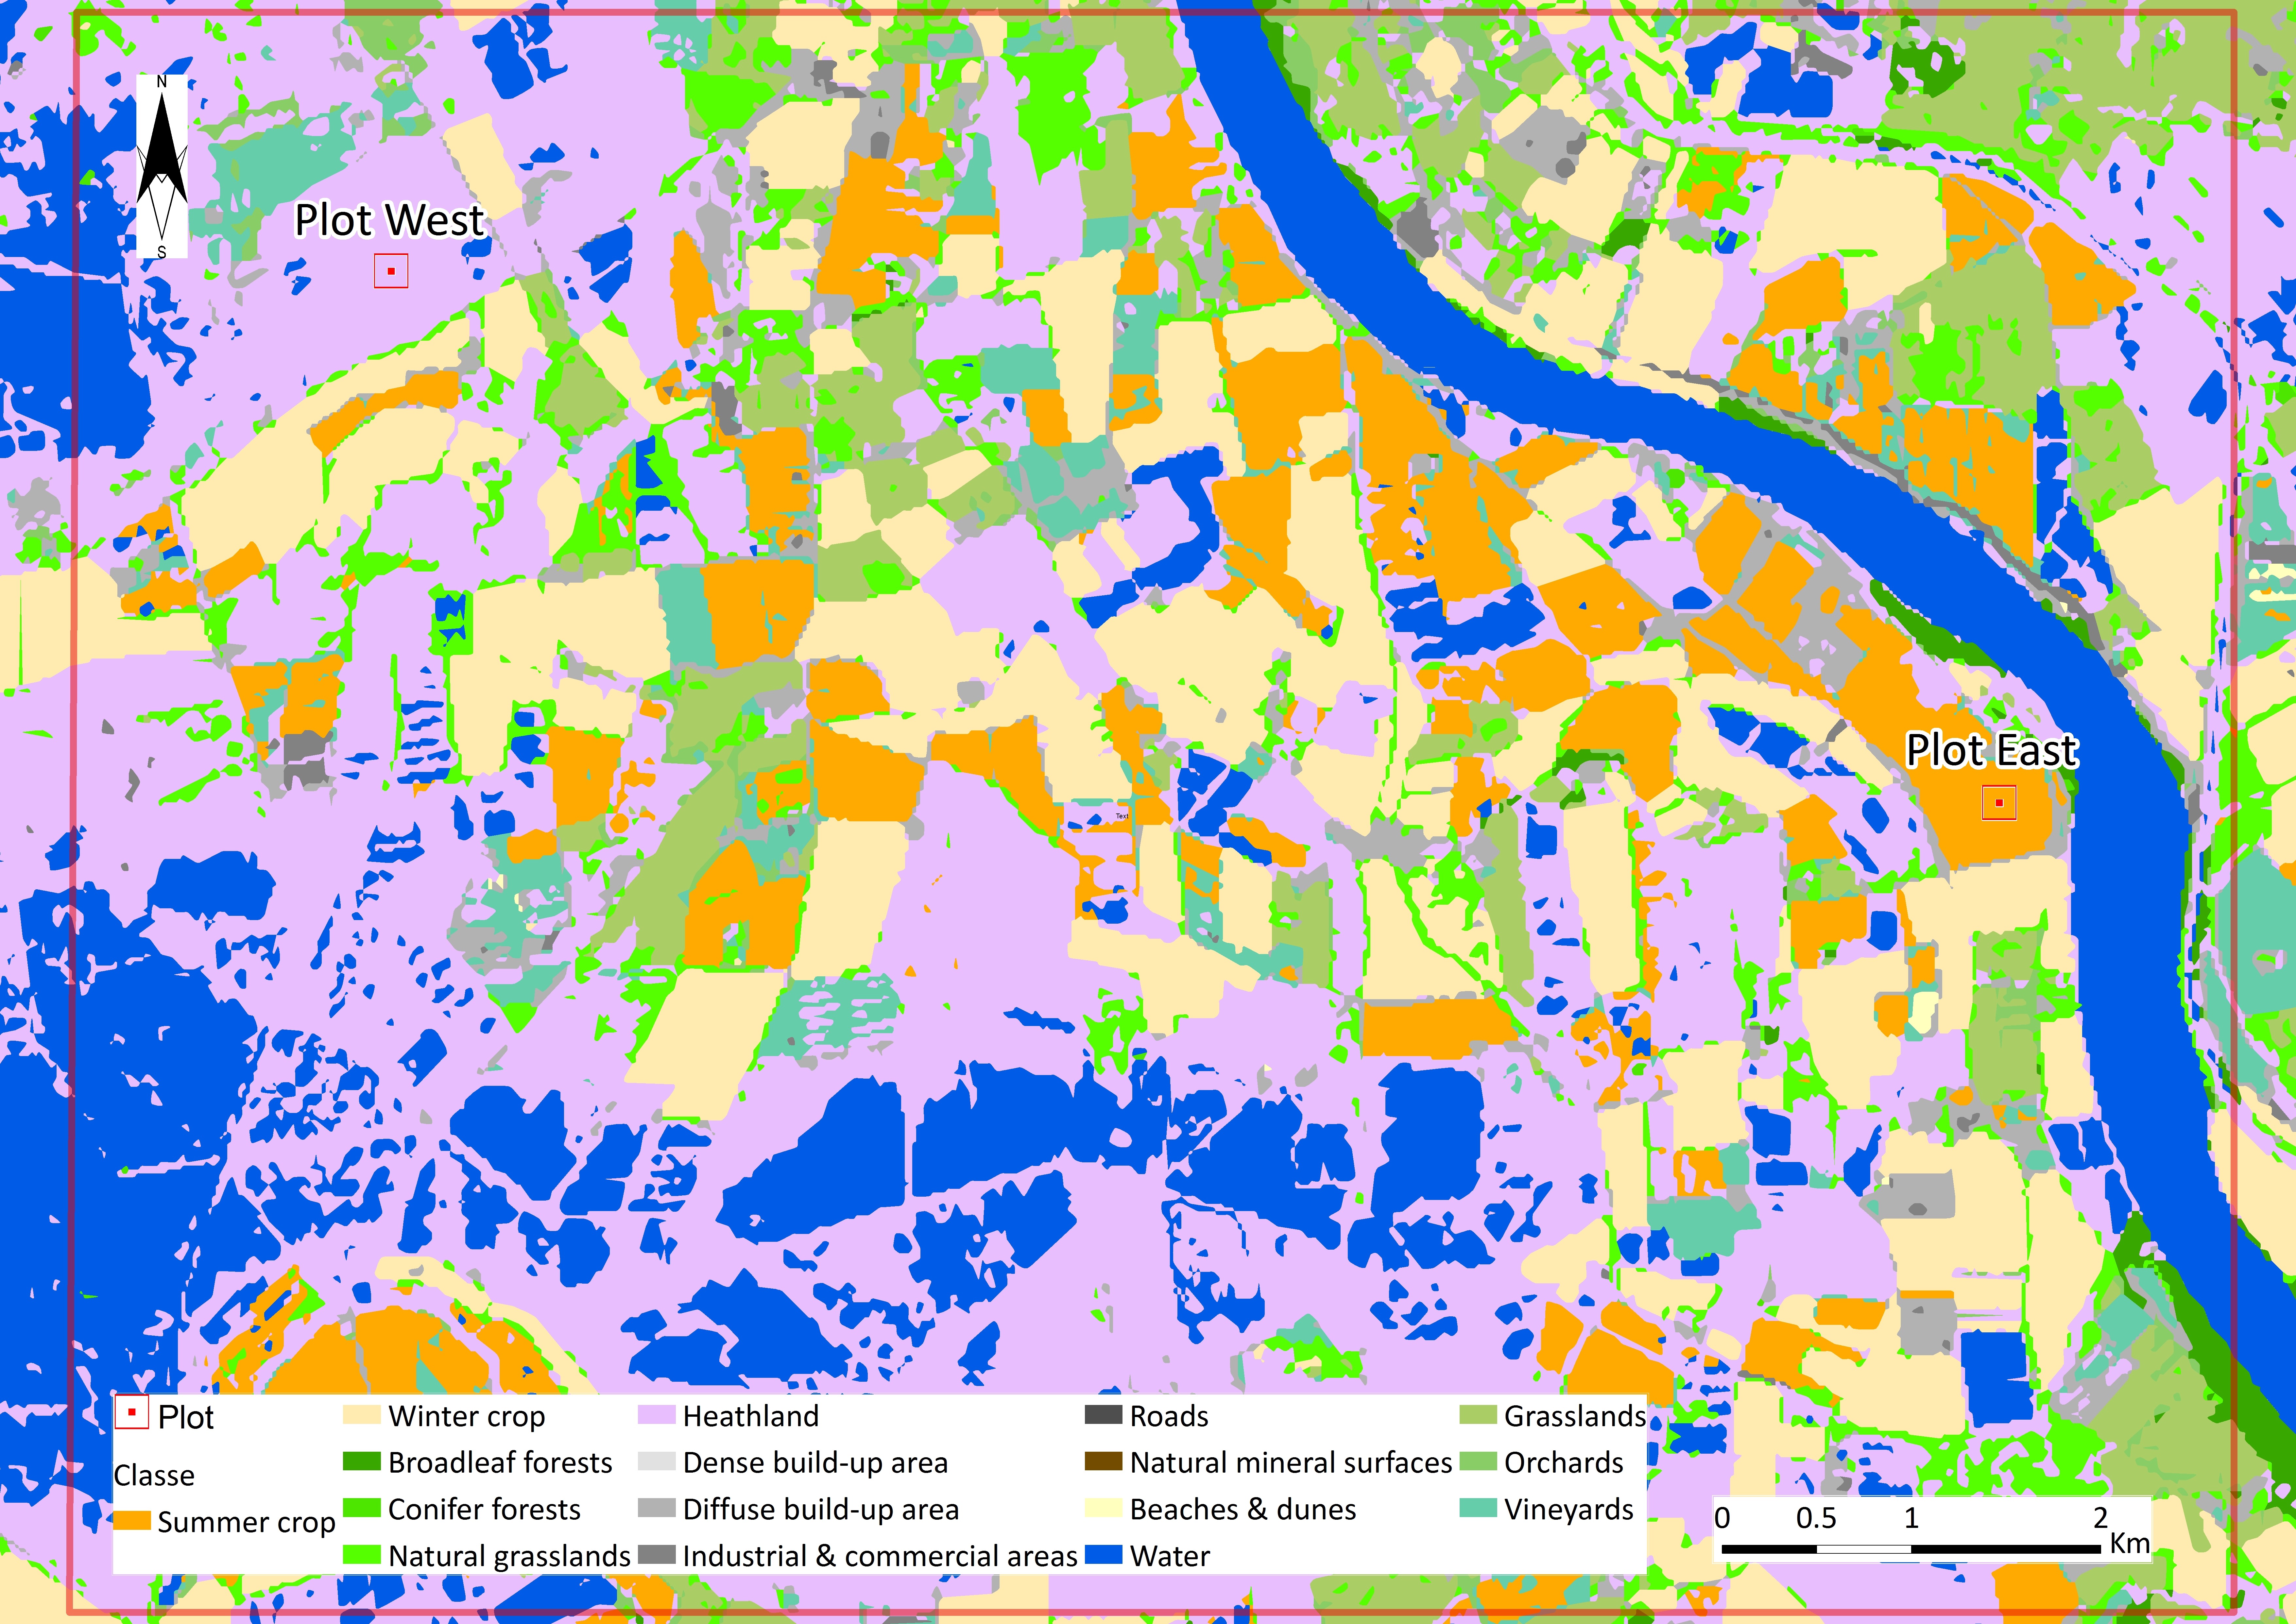
\includegraphics[width=8cm]{Figures/landcover_plot.jpg}
\caption{ROI with the two plots. Background: OSO Land Cover Map of 2016.}
\label{fig:twoplots}
\end{figure}

\begin{figure}[h]
\centering
\includegraphics[width=8cm]{Figures/Study area stats.png}
\caption{Largest land cover classes in the study site as of 2016 in ha (OSO)}
\label{fig:landcover}
\end{figure}



\section{MATERIAL AND METHODS}



\subsection{Raster Dataset}

The optical remote sensing satellite products we used were acquired from Landsat 7 and Landsat 8. One single optical image covers our study site (110 x 104 km) with a resolution of 30 m per pixel. Additionally, we used SAR data from Sentinel-1 to better detect open water areas. A detailed description of the satellite images we used is shown in table \ref{tab:table1}.

\begin{table}[htbp]
\centering
\includegraphics[width=8cm]{Figures/Table_datasets.png}
\caption{Time series and bands from Landsat 7 and 8 and Sentinel-1 we used for the paper.}
\label{tab:table1}
\end{table}


\subsection{Land Cover Dataset}
Land cover classes of the study area were acquired from the 2016 OSO Land Cover product of mainland France with 17 classes and a spatial resolution of 20 m. This dataset has a more detailed classification and higher update frequency compared to the CORINE dataset, which over-estimates rice field areas because it disregards the high crop rotation of rice \cite{Perennou2012ExistingOverview}.

\subsection{Indices}
In this paper, we used the indices NDVI, NDMI and LSWI to detect a seasonal pattern in irrigation and vegetation growth of rice fields in our study area.
\subsubsection{Vegetation Index}
To detect the peak of the vegetation growth and display greenness of agriculture, we used the Normalized difference vegetation index (NDVI), one of the most widely used vegetation index. Using the difference in reflectance between the NIR and Red band, the NDVI assesses the biomass, canopy structure, leaf area and chlorophyll content \cite{Rouse1974MonitoringSP-351}.
\begin{equation}
\label{eq:ndvi}
NDVI = \frac{\rho_{NIR}-\rho_{Red}}{\rho_{NIR}+\rho_{Red}}
\end{equation}

\subsubsection{Water Indices}

Normalized difference water index (NDWI) assesses plant water content, nitrogen content and surface waters \cite{Gao1996NDWISpace, McFeeters1996TheFeatures}. It lets water features stand out against soil and vegetation, which helps detecting the irrigated areas in spring.

\begin{equation}
NDWI = \frac{\rho_{Green}-\rho_{NIR}}{\rho_{Green}+\rho_{NIR}}    
\label{eq:ndwi}
\end{equation}

Comparison between LSWI and NDVI has been used as an important method to map the area of paddy rice fields \cite{Ryu2011AnalysisClassification}. In addition to NDWI, we calculate Land Surface Water Index (LSWI), which is sensitive to leaf water and soil moisture and therefore also an indicator for irrigated areas. 
\begin{equation}
\label{eq:lswi}
LSWI = \frac{\rho_{NIR}-\rho_{SWIR1}}{\rho_{NIR}+\rho_{SWIR1}}
\end{equation}



\subsubsection{Rice field Index}
We used an existing threshold \cite{Xiao2005MappingImages} to detect rice fields and called the resulting value Rice Field Index (RFI) for an easier understanding.
\begin{equation}
\label{eq:rfi}
RFI = {LSWI-NDVI+0.05}
\end{equation}


\subsection{Algorithm to identify rice fields}

Rice plants are grown on flooded soil with a water depth of 2 – 15 cm \cite{Xiao2005MappingImages}. The fields can be identified using the temporarily higher values of the LSWI compared to the NDVI during the irrigation period in spring. This works particularly in an agricultural context. We applied the method used by Xiao et al. (2005) who used the method to detect rice fields in South and Southeast Asia. The indices are combined in a manner that a simple threshold could be taken to detect the areas of interest (\ref{eq:rfi}). 

To confirm rice fields with an irrigation period, the results of the thresholding of Landsat 8 data with Sentinel-1 SAR data were combined. For that, the (preprocessed) Sentinel-1 data was transformed to dB and a threshold of -2 to extract water areas was applied.




\section{RESULTS}

\subsection{Identification of rice fields using the difference between LSWI and NDVI}

In figure (\ref{fig:waterdetection}) we can see that at the beginning of April 2015 in the agricultural area in the upper half of the scenery, only a few fields are masked and thus identified as rice fields. The number of masked fields increases throughout May. Also masked are the river Rhône and some areas in the lower part of the scenery which are, according to the OSO Land Cover Map, heathland, and smaller water bodies. This means natural areas with a lot of water around them are also classified. Some areas that were masked in April or May appear in saturated dark green in July and some of these areas reach an NDVI value of 0.9. Although these areas are still rice fields in July, they were not recognized as such by the mask. This means that our method recognizes the rice fields only if the water is visible. Therefore, we can say that the LSWI and NDVI combined approach worked best at the beginning of the growing season. Figure (\ref{fig:irrigation2015}) shows more detailed how the irrigation starts in some fields in April and extends until the mid of May.

\begin{figure}[h]
\centering
\includegraphics[width=8cm]{Figures/Water_detection_mask_2015.png}
\caption{Water detection mask of April–July 2015.}
\label{fig:waterdetection}
\end{figure}

\begin{figure}[h]
\centering
\includegraphics[width=8cm]{Figures/Irrigation_Period_2015.png}
\caption{Irrigation period of April–May 2015.}
\label{fig:irrigation2015}
\end{figure}

\subsection{Water detection with Sentinel-1 SAR images}

With the masked SAR images, it is possible to observe the irrigation of the agricultural areas spatially and temporally. Figure (\ref{fig:waterdetection}) shows that in agricultural areas water is mainly present in May in 2015. The only water bodies that are recognized permanently are the river Rhône and some smaller lakes and ponds in the lower part of the scenery that is heathland according to the OSO Land Cover Map.

\subsection{Relationship between irrigation and vegetation growth}
The indices show a clear seasonal pattern of water content and vegetation growth. The comparison between the NDWI and the NDVI shows how the irrigation period alternates with the growing period of vegetation. As soon as the growth reaches more than half maximum, the water detection gets more difficult and the NDWI signal gets weaker (see Appendix).

\subsection{Analysis of two smaller plots within the study site}
 
\subsubsection{Plot West}
The low SAR backscatter in spring of 2015, 2016 and 2017 (Figure \ref{fig:sarwest}) is indicative of an irrigation period as water surfaces have a low VH backscatter. This is supported by the indices and spectral signatures of the same dates (figures \ref{fig:ndviwest}, \ref{fig:lswiwest}, \ref{fig:ndwiwest} and \ref{fig:spectral2015}). In 2018 the lowest backscatter signals are later in the year which indicates that there was no rice cultivated that year. The harvest season is not detectable in the SAR backscatter.

The NDVI (Figure \ref{fig:ndviwest}) shows a clear seasonal pattern in all years. From 2015 to 2017 the minimum is in April followed by a peak in August and a minimum again at the end of November indicating the three periods of rice fields. In 2018 and 2019 the highest vegetation peak is in April and May, showing that there is a different crop in these years.

In the years of 2015 to 2019, the LSWI (Figure \ref{fig:lswiwest}) increases abruptly between April and May, then staying relatively constant throughout Summer to then gradually decrease again from September to November. This supports the classification of the plot as a rice field in these years. In 2018 and 2019, the LSWI shows a similar trend as the NDVI.

The NDWI (Figure \ref{fig:ndwiwest}) has its peaks in April and May in 2015 – 2017, also showing the irrigation period of the rice field nicely.

The RFI of Plot West (Figure \ref{fig:rfiwest}) clearly defines the area as a rice field from 2015–2017, where the values are above 0 during May.

\begin{figure}[h]
\centering
\includegraphics[width=8cm]{Figures/SAR_west.png}
\caption{SAR mean backscatter coefficient VH of Plot West from 2015–2018.}
\label{fig:sarwest}
\end{figure}

\begin{figure}[h]
\centering
\includegraphics[width=8cm]{Figures/LSWI-NDVI+0.05_west.png}
\caption{RFI of Plot West from 2015–2019.}
\label{fig:rfiwest}
\end{figure}

\subsubsection{Plot East}
The SAR backscatter signal is less distinct in the eastern plot, compared to Plot West (Figure \ref{fig:sareast}). In 2015 there is an overall higher backscatter signal that has a decreasing signal in May with an immediate strong increase in the end of May pointing to an irrigation period. The lowest values being at the end of June and August, however, speak against the classification as a rice field as harvest is normally between September and November. In 2016 there is a strong decrease of backscatter in May that points to an open water feature and therefore irrigation. There is however no visible harvest time in fall. In 2018 there are two cycles visible, one starting in February and the other starting in June. As rice fields typically are flooded in April or May, we can assume that those are different crop types. The indices and spectral signatures support this observation.

The NDVI (Figure \ref{fig:ndvieast}) shows two vegetation periods in 2015 and one in each of the other years. Only 2016 and 2019 can be rice fields, but the vegetation peaks are very late (September) which speaks against it. It seems that the field lies bare in spring both years based on the low NDVI values. This plot seems to have an alternation of two different crops. Yet, the cycle can’t be clearly defined with this short time span. The LSWI (Figure \ref{fig:lswieast}) shows the same trend as the NDVI.

The NDWI (Figure \ref{fig:ndwieast}) of the plot shows a clearer seasonality of water content than the SAR backscatter. It also shows that only in 2016 and 2019 there might have been irrigation in spring.

The RFI of Plot East (Figure \ref{fig:rfieast}) confirms that there is no year where the values are long enough above 0 to be sure that there is a rice field.

\begin{figure}[h]
\centering
\includegraphics[width=8cm]{Figures/SAR_east.png}
\caption{SAR mean backscatter coefficient VH of Plot East from 2015–2018.}
\label{fig:sareast}
\end{figure}

\begin{figure}[h]
\centering
\includegraphics[width=8cm]{Figures/LSWI-NDVI+0.05_east.png}
\caption{RFI of Plot East from 2015–2019.}
\label{fig:rfieast}
\end{figure}

\section{DISCUSSION}

In this paper we used indices derived from Landsat 7 and Landsat 8 combined with VH backscatter from Sentinel-1 to detect the rice fields and their irrigation cycle in the Camargue region. The approach was focusing on the three characteristic periods of rice fields that made them distinguishable from other land cover types. 

Like the studies that used MODIS \cite{Xiao2005MappingImages}, we experienced mixed spectral signals of water and vegetation during the growing season even though we used Landsat 8 images with a higher spatial resolution. This may have led to an under estimation of irrigated areas. The combination of LSWI and NDVI recognized flooded areas very reliably. But this method would not work successfully when applied to larger areas without preprocessing, because permanent water areas are detected too. Xiao et al. (2005) solved this issue by applying a permanent water mask on the area they studied. Since we looked only at two small plots in detail, we bypassed this issue. At some point in the growing period of vegetation (in the second half of June and therefore more than a month before yield) when the NDVI is between 0.5 and 0.7, the method does not recognize the rice fields as such anymore. This makes sense because by then the value of the NDVI will have decreased to the point where the final value falls below the threshold. Since the rice fields are not detected as such over their entire growing period, the time of the harvest cannot be observed using this method. Our approach using the difference between the LSWI and NDVI worked best at the beginning of the growing season where the crop has not covered the whole water area yet. The combination with the Sentinel-1 backscatter is used as validation of the classification, as it confirmed that irrigation occurred.

SAR backscatter thresholding to detect surface water works well in the specific agricultural context. It is very well possible to extract the irrigation period. In our case, this was helpful because of the higher temporal resolution and especially in years poor weather conditions in April and May. In an agricultural environment like the Camargue, where due to structural measures natural flooding have become rare and where rice the only crop is that grows in open water, a field can be classified with a high degree of certainty as a rice field due to irrigation.

In the way we used it, the SAR backscatter is only of value in the first part of the growing cycle. As the plants grow too far out of the water, the backscatter coefficient increases, and the area does not get recognized anymore. This is the case in the second half of May. Due to the advantage of not being weather-dependent, SAR data allows to monitor previously defined areas, even when the weather conditions are poor and observation with Landsat 8 would not be possible.The two plots we focused on were classified as rice (Plot East) and heathland (Plot West) by the OSO Land Cover Map, yet our approach classified Plot East as non-rice for most of the years (2015, 2017 & 2018). The RGB images of Landsat 8 showed that the plot often occurred white which could indicate a kind of artificial coverage as protection from birds or other animals. This would also explain the low NDVI in spring. The SAR thresholding detected irrigation of the field in spring of 2016 and in the winter of 2017/2018. 

Plot West is detected as rice from 2015 – 2017 by our approach. We can see the irrigation cycle and the following vegetation growth very well in the charts. In 2016, at the start of the growing season the rice field was recognized, but the following images were not usable due to cloudy weather conditions. As there is an irrigation cycle observed in the SAR backscatter and the field has a high NDVI in August, we can be confident that rice is planted in this year too. The same trend is visible for 2017. In 2018 the area was not recognized as a rice field by the Landsat 8 approach and there was no irrigation cycle visible, so we can assume that a different crop was cultivated that year. We expected rice to alternate half-yearly with a different crop (e.g., durum wheat), this seems to be the case in Plot West from 2015–2017. In Plot East there is also a half-yearly vegetation cycle visible, but it isn’t clear if it is rice as the indices don’t show a fitting signal. 

Further research would be necessary to refine the methods we applied. It would be important to find a way to classify the rice fields as such over the entire growing season. This would most likely be done also using spectral data. The SAR-method would need to become much more sophisticated so that it would be able to react to the changes of the signal. What would be of great use to develop more elaborate methods is more knowledge and information about the exact local conditions at specific times.




\section{CONCLUSIONS}
 
On agricultural areas, our combined methods were able to detect rice fields and their  cycle of irrigation from the flooding to the vegetation growth until harvest. The combination of different Landsat 7 and 8 indices is able to discriminate rice fields from other agricultural features. The SAR-method works very well to detect open water features. In previously defined areas, SAR data allows a weather-independent monitoring of the irrigation cycles of rice fields. This can be valuable, especially in years with poor weather conditions.  If there is basic knowledge about an area, how likely floodings are and which sort of crops could be cultivated, SAR data alone even works as reliable indicator of whether rice has been cultivated. The vegetation indices showed a clear signal over the whole period, the signal can be related meaningfully to the irrigation periods. For the Landsat 8-method and the SAR-method development would be needed to detect rice fields over their entire growing season which would make the method much more reliable.

   % This command serves to balance the column lengths
                                  % on the last page of the document manually. It shortens
                                  % the textheight of the last page by a suitable amount.
                                  % This command does not take effect until the next page
                                  % so it should come on the page before the last. Make
                                  % sure that you do not shorten the textheight too much.

%%%%%%%%%%%%%%%%%%%%%%%%%%%%%%%%%%%%%%%%%%%%%%%%%%%%%%%%%%%%%%%%%%%%%%%%%%%%%%%%



%%%%%%%%%%%%%%%%%%%%%%%%%%%%%%%%%%%%%%%%%%%%%%%%%%%%%%%%%%%%%%%%%%%%%%%%%%%%%%%%



%%%%%%%%%%%%%%%%%%%%%%%%%%%%%%%%%%%%%%%%%%%%%%%%%%%%%%%%%%%%%%%%%%%%%%%%%%%%%%%%
% \pagebreak







%%%%%%%%%%%%%%%%%%%%%%%%%%%%%%%%%%%%%%%%%%%%%%%%%%%%%%%%%%%%%%%%%%%%%%%%%%%%%%%%



\nocite{*}
\bibliographystyle{apacite}
\bibliography{references2}





\newpage

\section{APPENDIX}

\begin{figure}[h]
\centering
\includegraphics[width=8cm]{Figures/Spectral_profiles_2015_west.png}
\caption{Spectral profile of plot west in 2015 showing the three characteristic periods of rice fields.}
\label{fig:spectral2015}
\end{figure}

\begin{figure}[h]
\centering
\includegraphics[width=8cm]{Figures/NDVI_west.png}
\caption{NDVI of Plot West from 2015–2019.}
\label{fig:ndviwest}
\end{figure}

\begin{figure}[h]
\centering
\includegraphics[width=8cm]{Figures/LSWI_west.png}
\caption{LSWI of Plot West from 2015–2019.}
\label{fig:lswiwest}
\end{figure}

\begin{figure}[h]
\centering
\includegraphics[width=8cm]{Figures/NDWI_west.png}
\caption{NDWI of Plot West from 2015–2019.}
\label{fig:ndwiwest}
\end{figure}

\begin{figure}[h]
\centering
\includegraphics[width=8cm]{Figures/NDVI_east.png}
\caption{NDVI of Plot East from 2015–2019.}
\label{fig:ndvieast}
\end{figure}

\begin{figure}[h]
\centering
\includegraphics[width=8cm]{Figures/LSWI_east.png}
\caption{LSWI of Plot East from 2015–2019.}
\label{fig:lswieast}
\end{figure}

\begin{figure}[h]
\centering
\includegraphics[width=8cm]{Figures/NDWI_east.png}
\caption{NDWI of Plot East from 2015–2019.}
\label{fig:ndwieast}
\end{figure}

\end{document}